\chapter{FUNDAMENTAÇÃO TEÓRICA}
\label{cap:fundamentacao-teorica}
\section{Atividade Física e Parâmetros de Movimento em Cadeirantes}

\lipsum[1] \cite{AutorAno}. 

 Para \citeonline{AutorAno}, o \lipsum[1].

\lipsum[1]\cite{AutorAno}.

\lipsum[3]

\begin{figure}[H]
  \centering

  \begin{subfigure}[b]{0.45\textwidth}
    \centering
    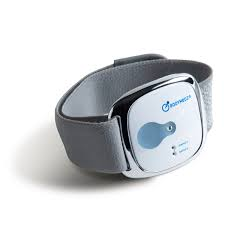
\includegraphics[height=5cm]{figuras/SenseWearArmband.jpeg}
    \caption{SenseWear\textsuperscript{\textregistered} Armband.}
    \fonte{\citeonline{bodymediaAmazon}}
    \label{fig:sensewear}
  \end{subfigure}
  \hfill
  \begin{subfigure}[b]{0.45\textwidth}
    \centering
    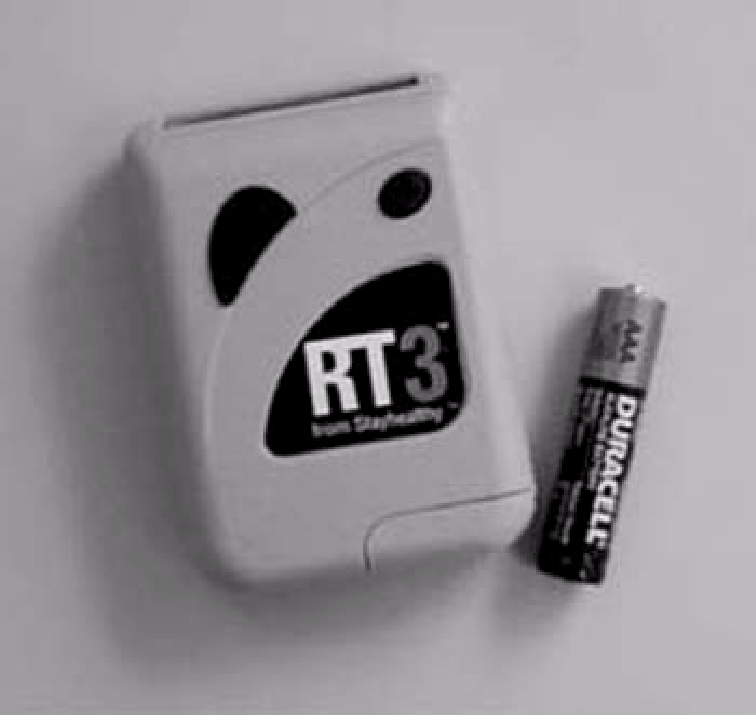
\includegraphics[height=5cm]{figuras/RT3.png}
    \caption{RT3 acelerômetro.}
    \fonte{\citeonline{FiguraR3}}
    \label{fig:rt3}
  \end{subfigure}

  \caption{Dispositivos vestíveis para monitoramento de atividade física: (a) SenseWear Armband e (b) RT3.}
  \label{fig:wearables}
\end{figure}

\lipsum[1]

\subsection{Tipos de lesão medular} 
% Diferenças funcionais entre LME traumática e deficiências Neurológicas não traumáticas}

Aqui uso de sigla \gls{TCC}, \gls{IFS} \lipsum[1].

\lipsum[6]


\section{Tecnologias Assistivas e Dispositivos Wearables}
\label{sec:Wearables}

\lipsum[6]


\subsection{Aplicativos para Esportes} %e a Utilização da Tecnologia a Favor do Usuário

\lipsum[1]

\lipsum[1]

\section{Inclusão Social e o Papel do Esporte}

\lipsum[4]

\lipsum[2]


\section{Informe aqui o título da section}
\lipsum[5]